As stated previously, the basic idea of lazy shadowing is to
associate a number of ``shadow processes'' with each main process. The
main responsibility of a shadow process is to take over the
responsibility of a failed main process and bring the computation to a
successful completion.  In this section, we define a framework for
evaluating lazy shadowing and then use this to derive a model for
representing the expected energy consumed by the system. %We then
%describe in terms of this model three different methods for applying
%lazy shadowing in a high performance computing environment.

%%model that describes and show how it can be used to derive the speed
%%of execution of the shadow process that minimizes energy
%%consumption. Without loss of generality, in this section, we focus on
%%the main process and its first shadow. The model can be easily
%%extended to deal with multiple shadows.

\subsection{Lazy Shadowing Framework}
\label{shadow_computing_framework}

The focus of this paper is on non-interactive batch jobs, such as scientific applications, financial analytics and image processing running on a large-scale HPC infrastructure. This class of applications is typically defined in terms of their workload, maximum resource consumption, and completion time, which varies from several hours to several days. They are usually delay tolerant and can be run anytime, as long as the target deadline is met. Each
application is composed of a large number of collaborative tasks. The
successful execution of the application depends on the successful
completion of all of these tasks. Therefore, the failure of a single
process delays the entire application, increasing the need for fault
tolerance. Each task must complete a specified amount of work, $W$, by
a targeted response time, $R$. The amount of work is expressed in
terms of the number of cycles required to complete the task. Each
computing node has a variable speed, $\sigma$, given in cycles per
second and bounded such that $0\leq\sigma\leq\sigma_{max}$. Therefore
the minimum response time for a given task is $R_{min}=W/\sigma_{max}$.

In order to achieve our desired fault tolerance a shadow process
executes in parallel with the main process on a different computing
node. The main process executes at a single execution speed denoted as
$\sigma_m$. In contrast the shadow process executes at two different
speeds, a speed before failure detection, $\sigma_b$, and a speed
after failure detection, $\sigma_a$. This is depicted in Figure
\ref{shadow_overview}.

\begin{figure}[hHtb]
\centering
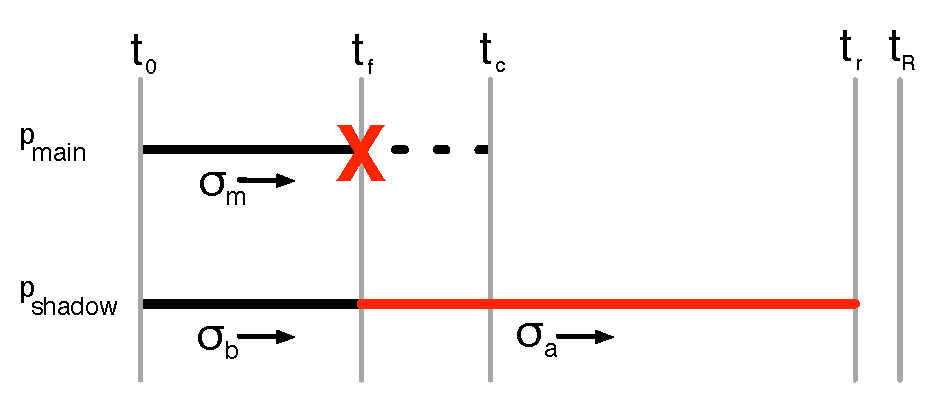
\includegraphics[width=\columnwidth]{figures/shadow_main_diagram.pdf}
%\psfig{figure=diagrams/shadow_main_diagram.eps,width=3.5in}
\caption { Overview of lazy shadowing.}
\label{shadow_overview}
\end{figure}


\subsection{Power Model}
\label{power_model}
Dynamic voltage and frequency scaling
(DVFS) has
been widely exploited as a technique to reduce CPU dynamic power~\cite{flautner_2002_APS,pillai_2001_sosp}.
It is well known that by varying the execution speed of the computing
nodes one can reduce their dynamic power consumption at least quadratically by
reducing their execution speed linearly. The power consumption of a
computing node executing at speed $\sigma$ is given by the function
$p_d(\sigma)$, represented by a polynomial of at least second degree,
$p_d(\sigma)=\sigma^n$ where $n\geq2$. 
In addition to the dynamic power, CPU leakage and other components
(memory, disk, network etc.) all contribute to static power
consumption, which is constant as long as the system is on. In this paper we
use $\rho$ to represent the weight of static power and $1-\rho$ the weight 
of dynamic power, when the node is running at the maximum speed.
Therefore, the power consumption is expressed as $p(\sigma)=\rho \times \sigma_{max}^n + (1-\rho)\times \sigma^n$.
The energy consumed by a
computing node executing at speed $\sigma$ during an interval of
length $T$ is given by $E(\sigma,T)=\int_{t=0}^T
p(\sigma)dt$. For an interval during which the speed is constant, the 
energy consumption can be calculated as $p(\sigma)t$. Throughout this paper
we assume that dynamic power is cubic in relation to speed, i.e., 
$p(\sigma)=\rho \times \sigma_{max}^3 + (1-\rho)\times \sigma^3$
We further assume that the computing node speed is bounded by the
following equation $0\leq\sigma\leq\sigma_{max}$.

\subsection{Failure Model}
\label{failure_model}

The failure can occur at any point during the execution of the main
task and the completed work is unrecoverable. Because the processes
are executing on different computing nodes we assume failures are
independent events. We also assume that only a single failure can
occur during the execution of a task. If the main task fails it is
therefore implied that the shadow will complete without failure. We
can make this assumption because we know the failure of any one node
is a rare event thus the failure of any two specific nodes is very
unlikely. In order to achieve higher resiliency one
would make use of multiple shadow processes and this failure model
will still be valid.

We assume that a probability density function, $f(t)$ ($\int_0^\infty
f(t)dt=1$), exists which expresses the probability of the main task
failing at time $t$. 
It is worth noting, that the lazy shadowing computation model 
does not depend on any specific distribution. However, in the remainder of this 
paper we use an exponential probability density function, $f(t) = \lambda e^{-\lambda t}$.
Numerous works have
studied the impact of DVFS on the failure rate or soft error rate
~\cite{firouzi2010reliability,zhu2004effects}. To take this effect into consideration,
we adopt the most widely used model from~\cite{zhu2004effects} and expressed it
within our framework as $\lambda(\sigma) = \lambda_0 10^{1-\sigma/\sigma_{max}}$. 
%Therefore, the failure distribution function is $f(\sigma, t) =  



\subsection{Energy Model}
\label{energy_model}

Given the power model and the failure distribution, the expected
energy consumed by a lazy shadowing task can be derived as the weighted
average considering all possible cases. 
First consider the case where no failure occurs and the main process
successfully completes the task at time $t_c^m$.
\begin{equation}
\begin{split}
E_1 = &  ( 1-\int_0^{t_c^m}f_m(t)dt) \times (1 - \int_0^{t_c^m} f_s(t)dt) \times \\
      &  (  E(\sigma_m,t_c^m) + E(\sigma_b,t_c^m))
\label{eq:energy_no_failure}
\end{split}
\end{equation}
The first line is the probability of fault-free execution of the main
process and shadow process. Then we multiple this probablity by the
energy consumed by the main and the shadow process during this fault
free execution, ending at $t_c^m$.

Next, consider the case where the shadow process fails at some point
before the main process successfully completes the task.
\begin{equation}
\begin{split}
E_2 = & (1-\int_0^{t_c^m}f_m(t)dt) \times \\
      & \int_0^{t_c^m}(E(\sigma_m,t_c^m)+E(\sigma_b,t)) \times f_s(t)dt
\label{eq:energy_shadow_fail}
\end{split}
\end{equation}
The first factor is the probability that the main process does not
fail, and the probability of shadow fails is included in the second factor which also contains the energy consumption since it depends on the shadow failure time. Energy consumption comes from the main process until the completion of the task,
and the shadow process before its failure.

The one remaining case to consider is when the main process fails and
the shadow process must continue to process until the task completes.
\begin{equation}
\begin{split}
E_3 = & (1-\int_0^{t_c^m}f_s(t)dt) \times \int_0^{t_c^m}(E(\sigma_m,t)+\\
      & E(\sigma_b,t)+E(\sigma_a,t_c^s-t))f_m(t)dt
\label{eq:energy_main_fail}
\end{split}
\end{equation}
Similarly, the first factor expresses the probability that the shadow process does
not fail. In this case, the shadow process executes from the beginning to
$t_c^s$ when it completes the task. However, under our ``at most one
failure'' assumption, the period during which shadow process may fail
ends at $t_c^m$, since the only reason why shadow process is still in
execution after $t_c^m$ is that main process has already failed. There
are three parts of energy consumption, including that of main process
before main's failure, that of shadow process before main's failure,
and that of shadow process after main's failure, all of which depend
on the failure occurrence time. 

By summing these three parts we will have
the expected energy consumed by lazy shadowing for completing a
task.
\begin{equation}
E[\text{energy}]= (E_1 + E_2 + E_3)
\label{eq:total_energy}
\end{equation}

\subsection{Optimization problem formulation}\

Using the models above we formulate our objective as the following
optimization problem.
%%% need more horizontal spacing here... not sure the latex-fu
\begin{equation}
\label{optimization_problem}
%\setlength{\abovedisplayskip}{14pt}
\begin{alignedat}{2}
\min_{\sigma_m,\sigma_b,\sigma_a}     & E[energy] \\
	s.t.							 & 0 \leq \sigma_m \leq \sigma_{max} \\
                                     & 0 \leq \sigma_b \leq \sigma_{m} \\
                                     & 0 \leq \sigma_a \leq \sigma_{max} \\
									 & t_m \leq t_R \\
									 & t_s \leq t_R	                                  
\end{alignedat}
\end{equation}

The first three constraints represent the physical limit on the execution speeds. 
The last two constraints guarantee that the task can be completed by the target 
response time both with and without failure.

It should be noted that it is assumed that node failures are unchangeable 
system properties and task
properties are given, therefore the system
parameters we can change are the execution speeds of the
processes. Thus, the output of this optimization problem is the
execution speeds, $\sigma_m$, $\sigma_b$ and $\sigma_a$. 

% LocalWords: hpc
